%% generato automaticamente da tools/build_tex.py --- non modificare
\chapter{Una delta di Dirac che vive nel piano complesso}
\label{cap:delta}
\quaderno{delta.dfw}{13 Jul 2010}{55}

Luglio 2010, cinquantacinque espressioni. È il quaderno più ambizioso della raccolta. Si parte da una famiglia di funzioni elementari che approssima la delta di Dirac; si osserva che la formula, scritta com'è, ha senso anche per argomento complesso; e si studia la funzione che ne risulta. Il finale tenta di usare quella funzione per dare un valore alla trasformata di Fourier di un esponenziale crescente, che nel senso ordinario non esiste. I conti sono corretti; come si vedrà, però, il valore ottenuto dipende dalla famiglia approssimante scelta, e non dalla delta.

\section{La famiglia approssimante}

Tutto il quaderno si regge su questa espressione, ripetuta decine di volte con argomenti sempre diversi. Conviene capirla subito, perché è molto più semplice di quanto sembri.

\begin{espr}{1}{Lim(User,n)}{}
\[
\lim_{n \to +\infty} \frac{1}{4}\, \left(\frac{1 + 2\, n\, x}{\left|x + \frac{1}{2\, n}\right|} + \frac{1 - 2\, n\, x}{\left|x - \frac{1}{2\, n}\right|}\right)
\]
\end{espr}
La famiglia approssimante: per ogni $n$ è un rettangolo alto $n$ e largo $1/n$, scritto senza usare definizioni a tratti.

\begin{figure}[htbp]
  \centering
  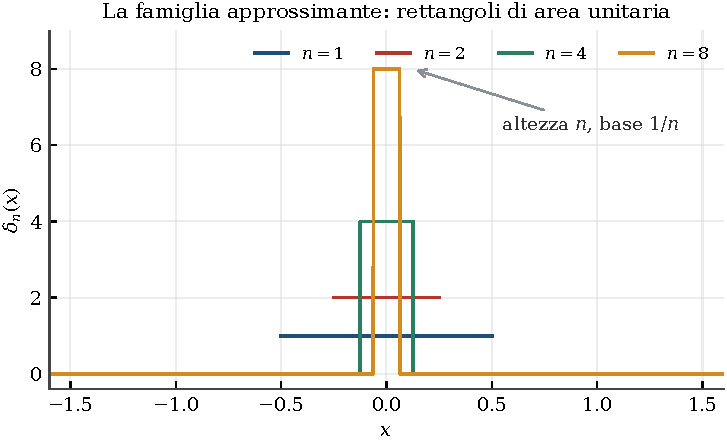
\includegraphics[width=0.86\linewidth]{../figures/delta_famiglia.pdf}
  \caption{La famiglia della riga $\#1$ per quattro valori di $n$. La formula, che non contiene definizioni a tratti, produce esattamente un rettangolo alto $n$ e largo $1/n$.}
  \label{fig:delta_famiglia}
\end{figure}
\begin{espr}{2}{User}{}
\begin{align*}
& \lim_{n \to +\infty} \int_{-\infty}^{+\infty} \frac{1}{4}\, \left(\frac{1 + 2\, n\, x}{\left|x + \frac{1}{2\, n}\right|} + \frac{1 - 2\, n\, x}{\left|x - \frac{1}{2\, n}\right|}\right) \,\mathrm{d}x \\
=\;& 1
\end{align*}
\end{espr}
L'area vale uno per ogni $n$, e quindi anche al limite.

\begin{figure}[htbp]
  \centering
  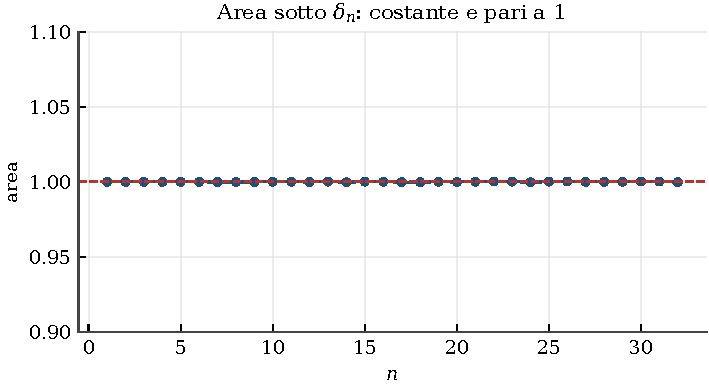
\includegraphics[width=0.86\linewidth]{../figures/delta_area.pdf}
  \caption{Verifica numerica della riga $\#2$: l'area resta uno al crescere di $n$, come deve essere per una famiglia che approssima la delta.}
  \label{fig:delta_area}
\end{figure}
\begin{espr}{3}{User}{}
\begin{align*}
& \lim_{n \to +\infty} \int_{-\infty}^{+\infty} \frac{1}{4}\, \left(\frac{1 + 2\, n\, \left(x - k\right)}{\left|x - k + \frac{1}{2\, n}\right|} + \frac{1 - 2\, n\, \left(x - k\right)}{\left|x - k - \frac{1}{2\, n}\right|}\right) \,\mathrm{d}x \\
=\;& 1
\end{align*}
\end{espr}
La stessa famiglia traslata nel punto $k$: l'area non cambia.


Per $x$ reale il calcolo si fa a mano. Se $|x|>1/(2n)$ i due valori assoluti si aprono con lo stesso segno e i due addendi valgono $+2n$ e $-2n$: la somma è nulla. Se invece $|x|<1/(2n)$ il secondo valore assoluto cambia segno e i due addendi valgono entrambi $2n$: la somma è $4n$, che diviso quattro dà $n$. Dunque
\[
  \delta_n(x)=\begin{cases} n & |x|<\dfrac{1}{2n}\\[6pt] 0 & \text{altrove,}\end{cases}
\]
cioè un rettangolo alto $n$ e largo $1/n$, di area unitaria per costruzione. È l'approssimante più semplice possibile della delta di Dirac, scritta però senza usare né la funzione segno né una definizione a tratti: solo valori assoluti e quozienti. La riga $\#2$ verifica l'area e la riga $\#3$ la trasla nel punto $k$.

\section{Che cosa succede con argomento complesso}

Qui comincia la parte originale. La formula della riga $\#1$ non contiene nulla che richieda un argomento reale: i valori assoluti si leggono come moduli, e tutto il resto è aritmetica. Che funzione si ottiene?

\begin{espr}{4}{User}{\verificata}
\begin{align*}
& \lim_{n \to +\infty} \frac{1}{4}\, \left(\frac{1 + 2\, n\, z}{\left|z + \frac{1}{2\, n}\right|} + \frac{1 - 2\, n\, z}{\left|z - \frac{1}{2\, n}\right|}\right) \\
=\;& \frac{z}{2\, \mathrm{i}\, \left|z\right|^{3}}\, \operatorname{Im}\!\left(z\right)
\end{align*}
\end{espr}
La formula centrale del quaderno. Con argomento complesso il limite non è una distribuzione ma una funzione ordinaria, definita ovunque tranne che nell'origine.

\begin{figure}[htbp]
  \centering
  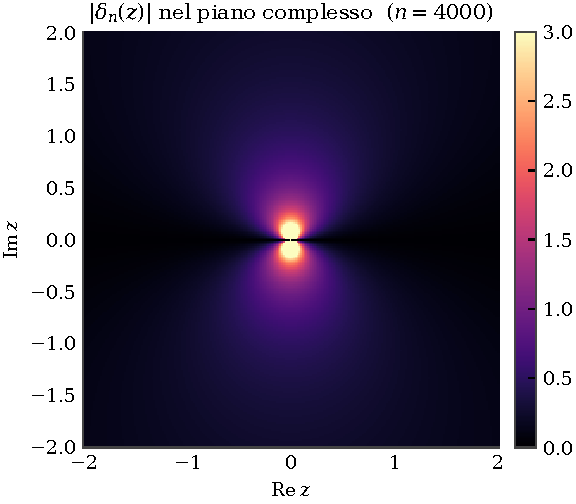
\includegraphics[width=0.62\linewidth]{../figures/delta_complesso.pdf}
  \caption{Il modulo della funzione della riga $\#4$ nel piano complesso. La linea scura lungo l'asse reale è il luogo $\operatorname{Im}z=0$, dove la funzione si annulla; i due lobi chiari sopra e sotto l'origine sono la singolarità $1/|z|$.}
  \label{fig:delta_complesso}
\end{figure}
\begin{espr}{5}{User}{\verificata}
\begin{align*}
& \lim_{n \to +\infty} \frac{1}{4}\, \left(\frac{1 + 2\, n\, \left(\mathrm{i}\, z\right)}{\left|\mathrm{i}\, z + \frac{1}{2\, n}\right|} + \frac{1 - 2\, n\, \left(\mathrm{i}\, z\right)}{\left|\mathrm{i}\, z - \frac{1}{2\, n}\right|}\right) \\
=\;& \frac{z}{2\, \left|z\right|^{3}}\, \operatorname{Re}\!\left(z\right)
\end{align*}
\end{espr}
Ruotando l'argomento di un quarto di giro, $\operatorname{Im}$ diventa $\operatorname{Re}$ e sparisce il fattore $\mathrm{i}$.

\begin{espr}{6}{User}{\verificata}
\begin{align*}
& \lim_{n \to +\infty} \frac{1}{4}\, \left(\frac{1 + 2\, n\, \left(\mathrm{i}\, z\right)}{\left|\mathrm{i}\, z + \frac{1}{2\, n}\right|} + \frac{1 - 2\, n\, \left(\mathrm{i}\, z\right)}{\left|\mathrm{i}\, z - \frac{1}{2\, n}\right|}\right) \\
&\qquad + \lim_{n \to +\infty} \frac{1}{4}\, \left(\frac{1 + 2\, n\, z}{\left|z + \frac{1}{2\, n}\right|} + \frac{1 - 2\, n\, z}{\left|z - \frac{1}{2\, n}\right|}\right) \\
=\;& \frac{1}{2\, \left|z\right|}
\end{align*}
\end{espr}
La somma delle due vale $1/(2|z|)$: si riconosce $z\bar z=|z|^2$.

\begin{espr}{7}{User}{\verificata}
\begin{align*}
& \lim_{n \to +\infty} \frac{1}{4}\, \left(\frac{1 + 2\, n\, \left(\mathrm{i}\, z\right)}{\left|\mathrm{i}\, z + \frac{1}{2\, n}\right|} + \frac{1 - 2\, n\, \left(\mathrm{i}\, z\right)}{\left|\mathrm{i}\, z - \frac{1}{2\, n}\right|}\right) \\
&\qquad - \lim_{n \to +\infty} \frac{1}{4}\, \left(\frac{1 + 2\, n\, z}{\left|z + \frac{1}{2\, n}\right|} + \frac{1 - 2\, n\, z}{\left|z - \frac{1}{2\, n}\right|}\right) \\
=\;& \frac{z^{2}}{2\, \left|z\right|^{3}}
\end{align*}
\end{espr}
La differenza vale $z^2/\left(2|z|^3\right)$.


La risposta della riga $\#4$ è la formula chiave di tutto il quaderno:
\[
  \delta(z)=\lim_{n\to\infty}\delta_n(z)=\frac{z\,\operatorname{Im}z}{2\mathrm{i}\,|z|^{3}}.
\]
Non è più un rettangolo: è una funzione definita su tutto il piano, che si annulla su tutto l'asse reale tranne che nell'origine — dove $\operatorname{Im}z=0$ — e che diverge come $1/|z|$ avvicinandosi all'origine dall'alto o dal basso. Il grafico del modulo ha la forma di un dipolo, con due lobi sopra e sotto lo zero e una linea di annullamento lungo i reali.

Le righe $\#5$--$\#7$ sono la parte che rende il tutto solido, e sono identità esatte. Ruotando l'argomento di un quarto di giro si ottiene la stessa formula con $\operatorname{Re}$ al posto di $\operatorname{Im}$ e senza il fattore $\mathrm{i}$; sommando le due si ottiene
\[
  \delta(\mathrm{i}z)+\delta(z)=\frac{z\left(\operatorname{Re}z-\mathrm{i}\operatorname{Im}z\right)}{2|z|^{3}}=\frac{z\bar z}{2|z|^{3}}=\frac{1}{2|z|},
\]
e sottraendole $\dfrac{z^2}{2|z|^{3}}$. Due righe, e la somma di due oggetti singolari diventa una funzione elementare del solo modulo.

\section{Come si comporta sotto riscalamento}

Le quattordici espressioni seguenti provano la formula su argomenti riscalati: per un fattore trigonometrico, per un fattore iperbolico, per un esponenziale immaginario. Tutte, lette con $\omega$ reale, sono esatte.

\begin{espr}{8}{User}{}
\begin{align*}
& \lim_{n \to +\infty} \frac{1}{4}\, \left(\frac{1 + 2\, n\, \left(z\, \cos\!\left(\omega\right)\right)}{\left|z\, \cos\!\left(\omega\right) + \frac{1}{2\, n}\right|} + \frac{1 - 2\, n\, \left(z\, \cos\!\left(\omega\right)\right)}{\left|z\, \cos\!\left(\omega\right) - \frac{1}{2\, n}\right|}\right) \\
=\;& \frac{\operatorname{Im}\!\left(z\right)\, z}{2\, \mathrm{i}\, \left|z\right|^{3}\, \left|\cos\!\left(\omega\right)\right|}
\end{align*}
\end{espr}
Riscalamento per $\cos\omega$: compare il fattore $1/|\cos\omega|$, esattamente come per la delta ordinaria.

\begin{espr}{9}{User}{}
\begin{align*}
& \lim_{n \to +\infty} \frac{1}{4}\, \left(\frac{1 + 2\, n\, \left(z\, \sin\!\left(\omega\right)\right)}{\left|z\, \sin\!\left(\omega\right) + \frac{1}{2\, n}\right|} + \frac{1 - 2\, n\, \left(z\, \sin\!\left(\omega\right)\right)}{\left|z\, \sin\!\left(\omega\right) - \frac{1}{2\, n}\right|}\right) \\
=\;& \frac{\operatorname{Im}\!\left(z\right)\, z}{2\, \mathrm{i}\, \left|z\right|^{3}\, \left|\sin\!\left(\omega\right)\right|}
\end{align*}
\end{espr}
Riscalamento per $\sin\omega$.

\begin{espr}{10}{User}{}
\begin{align*}
& \lim_{n \to +\infty} \frac{1}{4}\, \left(\frac{1 + 2\, n\, \left(z\, \cos\!\left(\mathrm{i}\, \omega\right)\right)}{\left|z\, \cos\!\left(\mathrm{i}\, \omega\right) + \frac{1}{2\, n}\right|} + \frac{1 - 2\, n\, \left(z\, \cos\!\left(\mathrm{i}\, \omega\right)\right)}{\left|z\, \cos\!\left(\mathrm{i}\, \omega\right) - \frac{1}{2\, n}\right|}\right) \\
=\;& \frac{\operatorname{Im}\!\left(z\right)\, \mathrm{e}^{\omega}\, z}{\mathrm{i}\, \left|z\right|^{3}\, \left(\mathrm{e}^{2\, \omega} + 1\right)}
\end{align*}
\end{espr}
Riscalamento per $\cos(\mathrm{i}\omega)=\cosh\omega$, scritto in forma esponenziale.

\begin{espr}{11}{User}{}
\begin{align*}
& \lim_{n \to +\infty} \frac{1}{4}\, \left(\frac{1 + 2\, n\, \left(z\, \sin\!\left(\mathrm{i}\, \omega\right)\right)}{\left|z\, \sin\!\left(\mathrm{i}\, \omega\right) + \frac{1}{2\, n}\right|} + \frac{1 - 2\, n\, \left(z\, \sin\!\left(\mathrm{i}\, \omega\right)\right)}{\left|z\, \sin\!\left(\mathrm{i}\, \omega\right) - \frac{1}{2\, n}\right|}\right) \\
=\;& \frac{\operatorname{Re}\!\left(z\right)\, \mathrm{e}^{\omega}\, z}{\left|z\right|^{3}\, \left|\mathrm{e}^{2\, \omega} - 1\right|}
\end{align*}
\end{espr}
Riscalamento per $\sin(\mathrm{i}\omega)=\mathrm{i}\sinh\omega$; il fattore $\mathrm{i}$ scambia $\operatorname{Im}$ con $\operatorname{Re}$.

\begin{espr}{12}{User}{\verificata}
\begin{align*}
& \lim_{n \to +\infty} \frac{1}{4}\, \left(\frac{1 + 2\, n\, \mathrm{e}^{\mathrm{i}\, z}}{\left|\mathrm{e}^{\mathrm{i}\, z} + \frac{1}{2\, n}\right|} + \frac{1 - 2\, n\, \mathrm{e}^{\mathrm{i}\, z}}{\left|\mathrm{e}^{\mathrm{i}\, z} - \frac{1}{2\, n}\right|}\right) \\
=\;& \frac{1}{2\, \mathrm{i}}\, \mathrm{e}^{\mathrm{i}\, \left(\operatorname{Re}\!\left(z\right) - \mathrm{i}\, \operatorname{Im}\!\left(z\right)\right)}\, \sin\!\left(\operatorname{Re}\!\left(z\right)\right)
\end{align*}
\end{espr}
Argomento sul cerchio unitario complesso.

\begin{espr}{13}{User}{}
\begin{align*}
& \lim_{n \to +\infty} \frac{1}{4}\, \left(\frac{1 + 2\, n\, \left(\mathrm{i}\, a\, \mathrm{e}^{\mathrm{i}\, z}\right)}{\left|\mathrm{i}\, a\, \mathrm{e}^{\mathrm{i}\, z} + \frac{1}{2\, n}\right|} + \frac{1 - 2\, n\, \left(\mathrm{i}\, a\, \mathrm{e}^{\mathrm{i}\, z}\right)}{\left|\mathrm{i}\, a\, \mathrm{e}^{\mathrm{i}\, z} - \frac{1}{2\, n}\right|}\right) \\
=\;& \frac{\mathrm{e}^{\mathrm{i}\, \left(\operatorname{Re}\!\left(z\right) - \mathrm{i}\, \operatorname{Im}\!\left(z\right)\right)}\, \cos\!\left(\operatorname{Re}\!\left(z\right)\right)}{2\, \left|a\right|}
\end{align*}
\end{espr}
Con un fattore $\mathrm{i}a$ davanti: compare $\cos$ al posto di $\sin$ e il modulo $|a|$ al denominatore.

\begin{espr}{14}{User}{}
\begin{align*}
& \lim_{n \to +\infty} \frac{1}{4}\, \left(\frac{1 + 2\, n\, \left(\mathrm{i}\, a\, \mathrm{e}^{\mathrm{i}\, z}\right)}{\left|\mathrm{i}\, a\, \mathrm{e}^{\mathrm{i}\, z} + \frac{1}{2\, n}\right|} + \frac{1 - 2\, n\, \left(\mathrm{i}\, a\, \mathrm{e}^{\mathrm{i}\, z}\right)}{\left|\mathrm{i}\, a\, \mathrm{e}^{\mathrm{i}\, z} - \frac{1}{2\, n}\right|}\right) \\
&\qquad + \lim_{n \to +\infty} \frac{1}{4}\, \left(\frac{1 + 2\, n\, \left(a\, \mathrm{e}^{\mathrm{i}\, z}\right)}{\left|a\, \mathrm{e}^{\mathrm{i}\, z} + \frac{1}{2\, n}\right|} + \frac{1 - 2\, n\, \left(a\, \mathrm{e}^{\mathrm{i}\, z}\right)}{\left|a\, \mathrm{e}^{\mathrm{i}\, z} - \frac{1}{2\, n}\right|}\right) \\
=\;& \frac{1}{2\, \left|a\right|}\, \mathrm{e}^{-\mathrm{i}\, \operatorname{Im}\!\left(z\right)}
\end{align*}
\end{espr}
La somma delle due versioni con e senza il fattore $\mathrm{i}$.

\begin{espr}{15}{User}{}
\begin{align*}
& \lim_{n \to +\infty} \frac{1}{4}\, \left(\frac{1 + 2\, n\, \left(\mathrm{i}\, a\, \mathrm{e}^{\mathrm{i}\, z}\right)}{\left|\mathrm{i}\, a\, \mathrm{e}^{\mathrm{i}\, z} + \frac{1}{2\, n}\right|} + \frac{1 - 2\, n\, \left(\mathrm{i}\, a\, \mathrm{e}^{\mathrm{i}\, z}\right)}{\left|\mathrm{i}\, a\, \mathrm{e}^{\mathrm{i}\, z} - \frac{1}{2\, n}\right|}\right) \\
&\qquad - \lim_{n \to +\infty} \frac{1}{4}\, \left(\frac{1 + 2\, n\, \left(a\, \mathrm{e}^{\mathrm{i}\, z}\right)}{\left|a\, \mathrm{e}^{\mathrm{i}\, z} + \frac{1}{2\, n}\right|} + \frac{1 - 2\, n\, \left(a\, \mathrm{e}^{\mathrm{i}\, z}\right)}{\left|a\, \mathrm{e}^{\mathrm{i}\, z} - \frac{1}{2\, n}\right|}\right) \\
=\;& \frac{1}{2\, \left|a\right|}\, \mathrm{e}^{\mathrm{i}\, 2\, \operatorname{Re}\!\left(z\right) + \operatorname{Im}\!\left(z\right)}
\end{align*}
\end{espr}
E la loro differenza.

\begin{espr}{16}{User}{}
\begin{align*}
& \lim_{n \to +\infty} \frac{1}{4}\, \left(\frac{1 + 2\, n\, \left(\mathrm{i}\, \mathrm{e}^{\mathrm{i}\, x}\right)}{\left|\mathrm{i}\, \mathrm{e}^{\mathrm{i}\, x} + \frac{1}{2\, n}\right|} + \frac{1 - 2\, n\, \left(\mathrm{i}\, \mathrm{e}^{\mathrm{i}\, x}\right)}{\left|\mathrm{i}\, \mathrm{e}^{\mathrm{i}\, x} - \frac{1}{2\, n}\right|}\right) \\
&\qquad + \lim_{n \to +\infty} \frac{1}{4}\, \left(\frac{1 + 2\, n\, \mathrm{e}^{\mathrm{i}\, x}}{\left|\mathrm{e}^{\mathrm{i}\, x} + \frac{1}{2\, n}\right|} + \frac{1 - 2\, n\, \mathrm{e}^{\mathrm{i}\, x}}{\left|\mathrm{e}^{\mathrm{i}\, x} - \frac{1}{2\, n}\right|}\right) \\
=\;& \frac{1}{2}
\end{align*}
\end{espr}
Il caso particolare $a=1$ con argomento reale: la somma vale $1/2$.

\begin{espr}{17}{User}{}
\begin{align*}
& \lim_{n \to +\infty} \frac{1}{4}\, \left(\frac{1 + 2\, n\, \left(\mathrm{i}\, \mathrm{e}^{\mathrm{i}\, \left(\frac{x}{2}\right)}\right)}{\left|\mathrm{i}\, \mathrm{e}^{\mathrm{i}\, \left(\frac{x}{2}\right)} + \frac{1}{2\, n}\right|} + \frac{1 - 2\, n\, \left(\mathrm{i}\, \mathrm{e}^{\mathrm{i}\, \left(\frac{x}{2}\right)}\right)}{\left|\mathrm{i}\, \mathrm{e}^{\mathrm{i}\, \left(\frac{x}{2}\right)} - \frac{1}{2\, n}\right|}\right) \\
&\qquad - \lim_{n \to +\infty} \frac{1}{4}\, \left(\frac{1 + 2\, n\, \mathrm{e}^{\mathrm{i}\, \left(\frac{x}{2}\right)}}{\left|\mathrm{e}^{\mathrm{i}\, \left(\frac{x}{2}\right)} + \frac{1}{2\, n}\right|} + \frac{1 - 2\, n\, \mathrm{e}^{\mathrm{i}\, \left(\frac{x}{2}\right)}}{\left|\mathrm{e}^{\mathrm{i}\, \left(\frac{x}{2}\right)} - \frac{1}{2\, n}\right|}\right) \\
=\;& \frac{1}{2}\, \mathrm{e}^{\mathrm{i}\, x}
\end{align*}
\end{espr}
Con argomento dimezzato: la differenza ricostruisce $\mathrm{e}^{\mathrm{i}x}/2$.

\begin{espr}{18}{User}{}
\begin{align*}
& \lim_{n \to +\infty} \frac{1}{4}\, \left(\frac{1 + 2\, n\, \mathrm{e}^{\mathrm{i}\, z}}{\left|\mathrm{e}^{\mathrm{i}\, z} + \frac{1}{2\, n}\right|} + \frac{1 - 2\, n\, \mathrm{e}^{\mathrm{i}\, z}}{\left|\mathrm{e}^{\mathrm{i}\, z} - \frac{1}{2\, n}\right|}\right) \\
&\qquad + \lim_{n \to +\infty} \frac{1}{4}\, \left(\frac{1 + 2\, n\, \mathrm{e}^{-\mathrm{i}\, z}}{\left|\mathrm{e}^{-\mathrm{i}\, z} + \frac{1}{2\, n}\right|} + \frac{1 - 2\, n\, \mathrm{e}^{-\mathrm{i}\, z}}{\left|\mathrm{e}^{-\mathrm{i}\, z} - \frac{1}{2\, n}\right|}\right) \\
=\;& \sin^{2}\!\left(z\right)
\end{align*}
\end{espr}
Somma delle versioni con esponenti coniugati: dà $\sin^2 z$.

\begin{espr}{19}{User}{}
\begin{align*}
& \lim_{n \to +\infty} \frac{1}{4}\, \left(\frac{1 + 2\, n\, \mathrm{e}^{\mathrm{i}\, z}}{\left|\mathrm{e}^{\mathrm{i}\, z} + \frac{1}{2\, n}\right|} + \frac{1 - 2\, n\, \mathrm{e}^{\mathrm{i}\, z}}{\left|\mathrm{e}^{\mathrm{i}\, z} - \frac{1}{2\, n}\right|}\right) \\
&\qquad - \lim_{n \to +\infty} \frac{1}{4}\, \left(\frac{1 + 2\, n\, \mathrm{e}^{-\mathrm{i}\, z}}{\left|\mathrm{e}^{-\mathrm{i}\, z} + \frac{1}{2\, n}\right|} + \frac{1 - 2\, n\, \mathrm{e}^{-\mathrm{i}\, z}}{\left|\mathrm{e}^{-\mathrm{i}\, z} - \frac{1}{2\, n}\right|}\right) \\
=\;& -\mathrm{i}\, \sin\!\left(z\right)\, \cos\!\left(z\right)
\end{align*}
\end{espr}
La differenza dà $-\mathrm{i}\sin z\cos z$, cioè metà del seno dell'angolo doppio.

\begin{espr}{20}{User}{}
\begin{align*}
& \lim_{n \to +\infty} \frac{1}{4}\, \left(\frac{1 + 2\, n\, \mathrm{i}\, \mathrm{e}^{\mathrm{i}\, z}}{\left|\mathrm{i}\, \mathrm{e}^{\mathrm{i}\, z} + \frac{1}{2\, n}\right|} + \frac{1 - 2\, n\, \mathrm{i}\, \mathrm{e}^{\mathrm{i}\, z}}{\left|\mathrm{i}\, \mathrm{e}^{\mathrm{i}\, z} - \frac{1}{2\, n}\right|}\right) \\
&\qquad - \lim_{n \to +\infty} \frac{1}{4}\, \left(\frac{1 + 2\, n\, \mathrm{i}\, \mathrm{e}^{-\mathrm{i}\, z}}{\left|\mathrm{i}\, \mathrm{e}^{-\mathrm{i}\, z} + \frac{1}{2\, n}\right|} + \frac{1 - 2\, n\, \mathrm{i}\, \mathrm{e}^{-\mathrm{i}\, z}}{\left|\mathrm{i}\, \mathrm{e}^{-\mathrm{i}\, z} - \frac{1}{2\, n}\right|}\right) \\
=\;& \mathrm{i}\, \sin\!\left(z\right)\, \cos\!\left(z\right)
\end{align*}
\end{espr}
Le stesse combinazioni con il fattore $\mathrm{i}$: la differenza cambia segno.

\begin{espr}{21}{User}{}
\begin{align*}
& \lim_{n \to +\infty} \frac{1}{4}\, \left(\frac{1 + 2\, n\, \mathrm{i}\, \mathrm{e}^{\mathrm{i}\, z}}{\left|\mathrm{i}\, \mathrm{e}^{\mathrm{i}\, z} + \frac{1}{2\, n}\right|} + \frac{1 - 2\, n\, \mathrm{i}\, \mathrm{e}^{\mathrm{i}\, z}}{\left|\mathrm{i}\, \mathrm{e}^{\mathrm{i}\, z} - \frac{1}{2\, n}\right|}\right) \\
&\qquad + \lim_{n \to +\infty} \frac{1}{4}\, \left(\frac{1 + 2\, n\, \mathrm{i}\, \mathrm{e}^{-\mathrm{i}\, z}}{\left|\mathrm{i}\, \mathrm{e}^{-\mathrm{i}\, z} + \frac{1}{2\, n}\right|} + \frac{1 - 2\, n\, \mathrm{i}\, \mathrm{e}^{-\mathrm{i}\, z}}{\left|\mathrm{i}\, \mathrm{e}^{-\mathrm{i}\, z} - \frac{1}{2\, n}\right|}\right) \\
=\;& \cos^{2}\!\left(z\right)
\end{align*}
\end{espr}
E la somma dà $\cos^2 z$. Con la riga $\#18$ si ottiene l'identità fondamentale.


Il meccanismo è sempre lo stesso, e si ricava dalla formula della riga $\#4$ in due passaggi. Se $c$ è una costante reale, allora $\operatorname{Im}(cz)=c\operatorname{Im}z$ e $|cz|=|c||z|$, per cui
\[
  \delta(cz)=\frac{cz\cdot c\operatorname{Im}z}{2\mathrm{i}\,|c|^3|z|^3}=\frac{1}{|c|}\,\delta(z).
\]
È la stessa regola di riscalamento della delta ordinaria, $\delta(cx)=\delta(x)/|c|$, e le righe $\#8$ e $\#9$ non fanno che scriverla con $c=\cos\omega$ e $c=\sin\omega$. Le righe $\#10$ e $\#11$ usano invece $\cos(\mathrm{i}\omega)=\cosh\omega$ e $\sin(\mathrm{i}\omega)=\mathrm{i}\sinh\omega$, e le forme che vi compaiono sono le stesse identità scritte con gli esponenziali: $1/\cosh\omega=2\mathrm{e}^{\omega}/\left(\mathrm{e}^{2\omega}+1\right)$ e $1/|\sinh\omega|=2\mathrm{e}^{\omega}/\left|\mathrm{e}^{2\omega}-1\right|$.

\section{La trasformata di un esponenziale crescente}

Questa è la sezione che giustifica tutto il lavoro precedente, ed è anche quella in cui la notazione del quaderno diventa più densa. La lettera $f$ indica un operatore di trasformazione applicato alla funzione che la segue, $\omega$ è la variabile trasformata, e $\delta$ è la funzione costruita nelle sezioni precedenti.

\begin{espr}{22}{User}{}
\begin{align*}
& f\, \mathrm{e}^{k\, t} \\
=\;& \delta\, \left(\omega + \mathrm{i}\, k\right) \\
=\;& \frac{k^{2} - \mathrm{i}\, k\, \omega}{2\, \mathrm{i}\, \left(k^{2} + \omega^{2}\right)^{\frac{3}{2}}}
\end{align*}
\end{espr}
La trasformata di $\mathrm{e}^{kt}$, scritta come delta valutata nel punto complesso $\omega+\mathrm{i}k$ e poi esplicitata con la formula della riga $\#4$.

\begin{espr}{23}{User}{}
\begin{align*}
& f\, \mathrm{e}^{-k\, t} \\
=\;& \delta\, \left(\omega - \mathrm{i}\, k\right) \\
=\;& \frac{k^{2} + \mathrm{i}\, k\, \omega}{2\, \mathrm{i}\, \left(k^{2} + \omega^{2}\right)^{\frac{3}{2}}}
\end{align*}
\end{espr}
Con l'esponente di segno opposto: la delta si sposta in $\omega-\mathrm{i}k$.

\begin{espr}{24}{User}{}
\[
\left|f\, \mathrm{e}^{k\, t}\right| = \left|f\, \mathrm{e}^{-k\, t}\right| = \frac{1}{2\, \left(\omega^{2} + 1\right)}
\]
\end{espr}
Il modulo comune delle due: per $k=1$ è la lorentziana $1/\left(2(\omega^2+1)\right)$.

\begin{espr}{25}{User}{}
\[
f\, \sinh\!\left(k\, t\right) = \frac{k^{2}}{2\, \left(k^{2} + \omega^{2}\right)^{\frac{3}{2}}}
\]
\end{espr}
La trasformata del seno iperbolico, cioè la semidifferenza delle due precedenti.

\begin{espr}{26}{User}{}
\[
f\, \cosh\!\left(k\, t\right) = \frac{-\mathrm{i}\, k\, \omega}{2\, \left(k^{2} + \omega^{2}\right)^{\frac{3}{2}}}
\]
\end{espr}
Quella del coseno iperbolico, cioè la semisomma.

\begin{espr}{27}{User}{}
\[
f\, \sinh\!\left(k\, t\right) = \frac{-\mathrm{i}\, \omega}{k}\, f\, \cosh\!\left(k\, t\right)
\]
\end{espr}
La relazione fra le due: differiscono per il fattore $-\mathrm{i}\omega/k$.


Il problema che questa sezione affronta è noto e serio. La trasformata di Fourier di $\mathrm{e}^{kt}$ non esiste: la funzione cresce e l'integrale diverge per ogni $\omega$ reale. Formalmente si scriverebbe $\delta(\omega+\mathrm{i}k)$ — una delta valutata in un punto complesso — ma nella teoria delle distribuzioni quella scrittura non ha significato, perché la delta è definita solo sui reali.

Qui il quaderno gliene attribuisce uno, perché la funzione $\delta(z)$ della riga $\#4$ è definita su tutto il piano. Sostituendovi $z=\omega+\mathrm{i}k$ si trova $\operatorname{Im}z=k$ e $|z|=\sqrt{k^2+\omega^2}$, da cui
\[
  \delta(\omega+\mathrm{i}k)=\frac{(\omega+\mathrm{i}k)\,k}{2\mathrm{i}\left(k^2+\omega^2\right)^{3/2}},
\]
che a meno del fattore $-\mathrm{i}$ è esattamente il secondo membro della riga $\#22$. La riga $\#24$ ne calcola il modulo e trova $1/\left(2(\omega^2+1)\right)$ per $k=1$: una lorentziana. Le righe $\#25$ e $\#26$ combinano i due segni per ottenere le trasformate del seno e del coseno iperbolico.

Qui però occorre una cautela che il quaderno non prende. Il valore di $\delta(z)$ fuori dall'asse reale non è una proprietà della delta ma della famiglia approssimante: con la famiglia lorentziana $\varepsilon/\left(\pi(z^2+\varepsilon^2)\right)$ il limite fuori dall'asse è $0$; con la gaussiana $\mathrm{e}^{-z^2/\varepsilon^2}/(\varepsilon\sqrt\pi)$ è $0$ dove $|\operatorname{Re}z|>|\operatorname{Im}z|$ e infinito dove $|\operatorname{Im}z|>|\operatorname{Re}z|$. Le trasformate di queste righe dipendono dunque dalla scelta del rettangolo. Nelle teorie in cui una delta in un punto complesso ha senso — i funzionali sulle funzioni test intere di Gel'fand e Šilov, le iperfunzioni di Sato — la delta non ha valori puntuali fuori dall'asse. La nota che accompagna questa edizione discute la questione per esteso.

\section{La proprietà di campionamento}

Tre integrali che verificano la proprietà per cui la delta esiste: setacciare il valore di una funzione in un punto.

\begin{espr}{28}{User}{}
\begin{align*}
& \lim_{n \to +\infty} \int_{-\infty}^{+\infty} \frac{\mathrm{e}^{x + 1}}{4}\, \left(\frac{1 + 2\, n\, x}{\left|x + \frac{1}{2\, n}\right|} + \frac{1 - 2\, n\, x}{\left|x - \frac{1}{2\, n}\right|}\right) \,\mathrm{d}x \\
=\;& \mathrm{e}
\end{align*}
\end{espr}
La proprietà di campionamento: l'integrale estrae il valore di $\mathrm{e}^{x+1}$ nell'origine.

\begin{espr}{29}{User}{}
\begin{align*}
& \lim_{n \to +\infty} \int_{-\infty}^{+\infty} \frac{\mathrm{e}^{x}}{4}\, \left(\frac{1 + 2\, n\, \left(x - 1\right)}{\left|x - 1 + \frac{1}{2\, n}\right|} + \frac{1 - 2\, n\, \left(x - 1\right)}{\left|x - 1 - \frac{1}{2\, n}\right|}\right) \,\mathrm{d}x \\
=\;& \mathrm{e}
\end{align*}
\end{espr}
Con la delta traslata in $1$: si estrae $\mathrm{e}^1$.

\begin{espr}{30}{User}{}
\begin{align*}
& \lim_{n \to +\infty} \int_{-\infty}^{+\infty} \frac{\mathrm{e}^{x}}{4}\, \left(\frac{1 + 2\, n\, \left(\frac{x}{3} - 4\right)}{\left|\frac{x}{3} - 4 + \frac{1}{2\, n}\right|} + \frac{1 - 2\, n\, \left(\frac{x}{3} - 4\right)}{\left|\frac{x}{3} - 4 - \frac{1}{2\, n}\right|}\right) \,\mathrm{d}x \\
=\;& 3\, \mathrm{e}^{12}
\end{align*}
\end{espr}
Con argomento riscalato e traslato: lo zero è in $x=12$ e il fattore di scala $1/3$ produce il $3$ davanti.

\begin{espr}{31}{User}{}
\begin{align*}
& \lim_{e \to 0} \lim_{n \to +\infty} \int_{-e}^{+e} 4\, \left(\frac{1 + 2\, n\, x}{\left|x + \frac{1}{2\, n}\right|} + \frac{1 - 2\, n\, x}{\left|x - \frac{1}{2\, n}\right|}\right)^{-1} \,\mathrm{d}x \\
=\;& 0
\end{align*}
\end{espr}
L'integrale del reciproco su un intervallo che si stringe: tende a zero.

\begin{espr}{32}{User}{}
\begin{align*}
& \lim_{e \to 0} \lim_{n \to +\infty} \int_{-\infty}^{+\infty} 4\, \left(\frac{1 + 2\, n\, x}{\left|x + \frac{1}{2\, n}\right|} + \frac{1 - 2\, n\, x}{\left|x - \frac{1}{2\, n}\right|}\right)^{-1} \,\mathrm{d}x \\
=\;& \pm \infty
\end{align*}
\end{espr}
Sull'intera retta invece diverge, con segno indeterminato.


Le tre righe sono corrette e la terza è la più istruttiva. L'argomento $x/3-4$ si annulla in $x=12$, ma con derivata $1/3$: la regola $\delta(ax+b)=\delta\!\left(x+b/a\right)/|a|$ dà quindi un fattore $3$, e il risultato è $3\,\mathrm{e}^{12}$ come scritto. È la proprietà di riscalamento della sezione precedente, applicata sotto integrale.

Le righe $\#31$ e $\#32$ fanno la prova opposta: integrano il \emph{reciproco} della famiglia approssimante. Su un intervallo che si stringe attorno all'origine il risultato è zero, perché lì la funzione vale $1/n$; su tutta la retta diverge, perché fuori dal rettangolo il reciproco è infinito.

\section{Le derivate della delta complessa}

Cinque righe che elencano le derivate successive della funzione della riga $\#4$. Il quaderno le scrive senza commento; conviene guardare i coefficienti.

\begin{espr}{33}{User}{}
\[
\lim_{n \to +\infty} \frac{1}{4}\, \left(\frac{1 + 2\, n\, x}{\left|x + \frac{1}{2\, n}\right|} + \frac{1 - 2\, n\, x}{\left|x - \frac{1}{2\, n}\right|}\right)
\]
\end{espr}
La funzione limite, ripetuta come punto di partenza per le derivate.

\begin{espr}{34}{User}{}
\[
\frac{\mathrm{i}}{\left|z\right|^{3}}\, \operatorname{Im}\!\left(z\right)
\]
\end{espr}
Derivata prima.

\begin{espr}{35}{User}{}
\[
\frac{3\, \left|z\right|\, \operatorname{Im}\!\left(z\right)}{\mathrm{i}\, z^{5}}
\]
\end{espr}
Derivata seconda.

\begin{espr}{36}{User}{}
\[
\frac{12\, \mathrm{i}\, \operatorname{Im}\!\left(z\right)}{\left|z\right|^{5}}
\]
\end{espr}
Derivata terza: il coefficiente è $12$.

\begin{espr}{37}{User}{}
\[
\frac{60\, z\, \operatorname{Im}\!\left(z\right)}{\mathrm{i}\, z^{7}}
\]
\end{espr}
Derivata quarta: $60$.

\begin{espr}{38}{User}{}
\[
\frac{360\, \mathrm{i}\, \operatorname{Im}\!\left(z\right)}{z^{7}}
\]
\end{espr}
Derivata quinta: $360$. La successione $1,3,12,60,360$ è $(n+2)!/2$.


I coefficienti sono $1,\ 3,\ 12,\ 60,\ 360$, e ciascuno è il precedente moltiplicato per $3,4,5,6$: si tratta di $(n+2)!/2$. È la stessa struttura fattoriale che hanno le derivate della delta ordinaria nella teoria delle distribuzioni, dove $\delta^{(n)}$ agisce estraendo la derivata $n$-esima della funzione di prova con un fattore $(-1)^n n!$.

\section{Il ritorno alla parametrizzazione del cerchio}

Le ultime righe cambiano registro. C'è un calcolo isolato che non c'entra con il resto, e poi il quaderno torna sulla sostituzione di Weierstrass, la stessa che due mesi dopo sarà il tema di \dfw{gauss.dfw}.

\begin{espr}{39}{Sum(User,x)}{}
\[
\sum_{x=-5}^{5} \sin\!\left(\cos\!\left(n\, x\right)\right)
\]
\end{espr}
Un calcolo isolato, senza rapporto con il resto del quaderno.

\begin{espr}{40}{Simp(\#39)}{}
\begin{align*}
& 2\, \sin\!\left(\cos\!\left(5\, n\right)\right) + 2\, \sin\!\left(\cos\!\left(4\, n\right)\right) + 2\, \sin\!\left(\cos\!\left(3\, n\right)\right) + 2\, \sin\!\left(\cos\!\left(2\, n\right)\right) \\
&\qquad + 2\, \sin\!\left(\cos\!\left(n\right)\right) + \sin\!\left(1\right)
\end{align*}
\end{espr}
Il risultato: la somma è simmetrica e i termini si raddoppiano tranne quello centrale.

\begin{espr}{41}{User}{}
\begin{align*}
& \mathrm{e}^{2\, \mathrm{i}\, x} \\
=\;& \operatorname{sgn}^{2}\!\left(1 + \mathrm{i}\, \tan\!\left(x\right)\right) \\
=\;& \left(\frac{1 + \mathrm{i}\, \tan\!\left(x\right)}{\left|1 + \mathrm{i}\, \tan\!\left(x\right)\right|}\right)^{2} \\
=\;& \frac{\left(1 + \mathrm{i}\, \tan\!\left(x\right)\right)^{2}}{1 + \tan^{2}\!\left(x\right)}
\end{align*}
\end{espr}
La sostituzione di Weierstrass, in quattro scritture equivalenti.

\begin{espr}{42}{User}{}
\begin{align*}
& \lim_{n \to +\infty} \frac{1}{4}\, \left(\frac{1 + 2\, n\, \left(1 + \mathrm{i}\, \tan\!\left(x\right)\right)}{\left|1 + \mathrm{i}\, \tan\!\left(x\right) + \frac{1}{2\, n}\right|} + \frac{1 - 2\, n\, \left(1 + \mathrm{i}\, \tan\!\left(x\right)\right)}{\left|1 + \mathrm{i}\, \tan\!\left(x\right) - \frac{1}{2\, n}\right|}\right) \\
=\;& \frac{\mathrm{e}^{\mathrm{i}\, x}\, \sin\!\left(x\right)\, \left|\cos\!\left(x\right)\right|}{2\, \mathrm{i}}
\end{align*}
\end{espr}
La famiglia approssimante applicata al numero che parametrizza il cerchio.

\begin{espr}{43}{User}{}
\begin{align*}
& \mathrm{e}^{\mathrm{i}\, x} \\
=\;& \frac{-\sin\!\left(x\right)\, \left|\cos\!\left(x\right)\right|\, \left(1 + \mathrm{i}\, \tan\!\left(x\right)\right)}{\cos^{2}\!\left(x\right)\, \left|1 + \tan\!\left(x\right)\right|}
\end{align*}
\end{espr}
Una riscrittura dell'esponenziale immaginario che ne discende.

\begin{espr}{44}{User}{}
\[
\frac{\left(1 + \mathrm{i}\, \tan\!\left(\frac{x}{2}\right)\right)^{2}}{1 + \tan^{2}\!\left(\frac{x}{2}\right)}
\]
\end{espr}
La parametrizzazione con argomento dimezzato.

\begin{espr}{45}{User}{}
\[
\lim_{x \to \frac{\pi}{2}} \tan\!\left(x\right) = \mathrm{i}
\]
\end{espr}
Nel senso ordinario il limite non esiste: la tangente diverge con segni opposti dai due lati. La scrittura va letta come limite dell'argomento di $1+\mathrm{i}\tan x$, che tende a $\pi/2$.

\begin{espr}{46}{User}{}
\[
\int \frac{1}{2\, \left(\omega^{2} + 1\right)^{\frac{3}{2}}} \,\mathrm{d}\omega = \frac{\omega}{2\, \sqrt{\omega^{2} + 1}}
\]
\end{espr}
Un integrale elementare corretto, che serve alla sezione sulle trasformate.

\begin{espr}{47}{User}{}
\[
\int \frac{-\mathrm{i}\, \omega}{2\, \left(\omega^{2} + 1\right)^{\frac{3}{2}}} \,\mathrm{d}\omega = \frac{\mathrm{i}}{2\, \sqrt{\omega^{2} + 1}}
\]
\end{espr}
Il suo compagno con il fattore immaginario.

\begin{espr}{48}{User}{\verificata}
\[
\cosh^{2}\!\left(t\right) + \sinh^{2}\!\left(t\right) = \cosh\!\left(2\, t\right)
\]
\end{espr}
L'identità di duplicazione iperbolica.

\begin{espr}{49}{User}{\verificata}
\[
\cosh^{2}\!\left(t\right) - \sinh^{2}\!\left(t\right) = 1
\]
\end{espr}
E quella fondamentale.

\begin{espr}{50}{User}{}
\[
f\, \cosh^{2}\!\left(t\right) = \frac{\omega}{2\, \mathrm{i}\, \left(4 + \omega^{2}\right)^{\frac{3}{2}}} + \pi\, \delta
\]
\end{espr}
La trasformata del coseno iperbolico al quadrato: compare un termine $\pi\delta$, che è la componente continua.

\begin{espr}{51}{User}{}
\[
f\, \sinh^{2}\!\left(t\right) = \frac{\omega}{2\, \mathrm{i}\, \left(4 + \omega^{2}\right)^{\frac{3}{2}}} - \pi\, \delta
\]
\end{espr}
Quella del seno iperbolico al quadrato, con il termine $\pi\delta$ di segno opposto.

\begin{espr}{52}{User}{}
\[
\int_{0}^{+\infty} \frac{\cos\!\left(\omega\, t\right) + \omega\, \sin\!\left(\omega\, t\right)}{\left(\omega^{2} + 1\right)^{\frac{3}{2}}} \,\mathrm{d}\omega
\]
\end{espr}
L'integrale di inversione, su tutta la semiretta.

\begin{espr}{53}{User}{}
\[
\int_{0}^{99999999} \frac{\cos\!\left(\omega\, t\right) + \omega\, \sin\!\left(\omega\, t\right)}{\left(\omega^{2} + 1\right)^{\frac{3}{2}}} \,\mathrm{d}\omega
\]
\end{espr}
Troncato a $10^8$.

\begin{espr}{54}{User}{}
\[
\int_{0}^{999} \frac{\cos\!\left(\omega\, t\right) + \omega\, \sin\!\left(\omega\, t\right)}{\left(\omega^{2} + 1\right)^{\frac{3}{2}}} \,\mathrm{d}\omega
\]
\end{espr}
Troncato a $999$: le due righe misurano quanto lentamente converge.

\begin{espr}{55}{User}{}
\[
\frac{\cos\!\left(\omega\, t\right) + \omega\, \sin\!\left(\omega\, t\right)}{\left(\omega^{2} + 1\right)^{\frac{3}{2}}}
\]
\end{espr}
L'integrando isolato.


Due osservazioni finali. La riga $\#45$ scrive che il limite della tangente in $\pi/2$ vale $\mathrm{i}$: nel senso ordinario quel limite non esiste, perché la tangente diverge con segni opposti dai due lati. Nel contesto delle righe che la circondano, però, la scrittura è comprensibile: quello che tende a $\mathrm{i}$ è $\mathrm{sgn}\!\left(1+\mathrm{i}\tan x\right)$, il cui argomento tende a $\pi/2$. È la stessa abbreviazione già incontrata in \dfw{j.dfw} (capitolo~\ref{cap:j}).

Le righe $\#48$--$\#51$ chiudono invece con una verifica di coerenza che funziona perfettamente. Poiché $\cosh^2t-\sinh^2t=1$ e la trasformata della costante $1$ è $2\pi\delta$, la differenza fra le trasformate delle righe $\#50$ e $\#51$ deve valere $2\pi\delta$ — e infatti i termini in $\omega$ si cancellano e restano esattamente $\pi\delta+\pi\delta$. Analogamente, $\cosh^2t+\sinh^2t=\cosh2t$, e la somma delle due trasformate dà una funzione di $\omega$ in cui compare $4=2^2$: la frequenza è raddoppiata, come deve essere.

\section*{In sintesi}
\addcontentsline{toc}{section}{In sintesi}

Il quaderno prende una formula elementare per la delta di Dirac, la valuta in un punto complesso, e trova una funzione ordinaria: $\delta(z)=z\operatorname{Im}(z)/\left(2\mathrm{i}|z|^3\right)$, metà della derivata lungo l'asse reale del segno complesso $z/|z|$. Questa funzione si annulla sull'asse reale, obbedisce alla stessa regola di riscalamento della delta ordinaria e ha derivate con coefficienti fattoriali. Il quaderno la usa per dare un valore a $\delta(\omega+\mathrm{i}k)$, cioè alla trasformata di Fourier dell'esponenziale crescente; ma quel valore dipende dalla famiglia approssimante — con la lorentziana sarebbe nullo, con la gaussiana non esisterebbe — e nelle teorie rigorose, i funzionali analitici e le iperfunzioni, la delta non ha valori puntuali fuori dall'asse.

I conti sono corretti; l'interpretazione no. Le verifiche di coerenza delle righe $\#50$ e $\#51$ usano solo la linearità, e valgono per qualunque famiglia. Resta una domanda legittima, che il quaderno pone senza saperlo: c'è un senso in cui la famiglia a rettangolo sia quella giusta?

